% !TeX root = ICCPS18.tex
   
     \begin{figure}[t]
 \centering
\resizebox{0.45\textwidth}{!}{%
 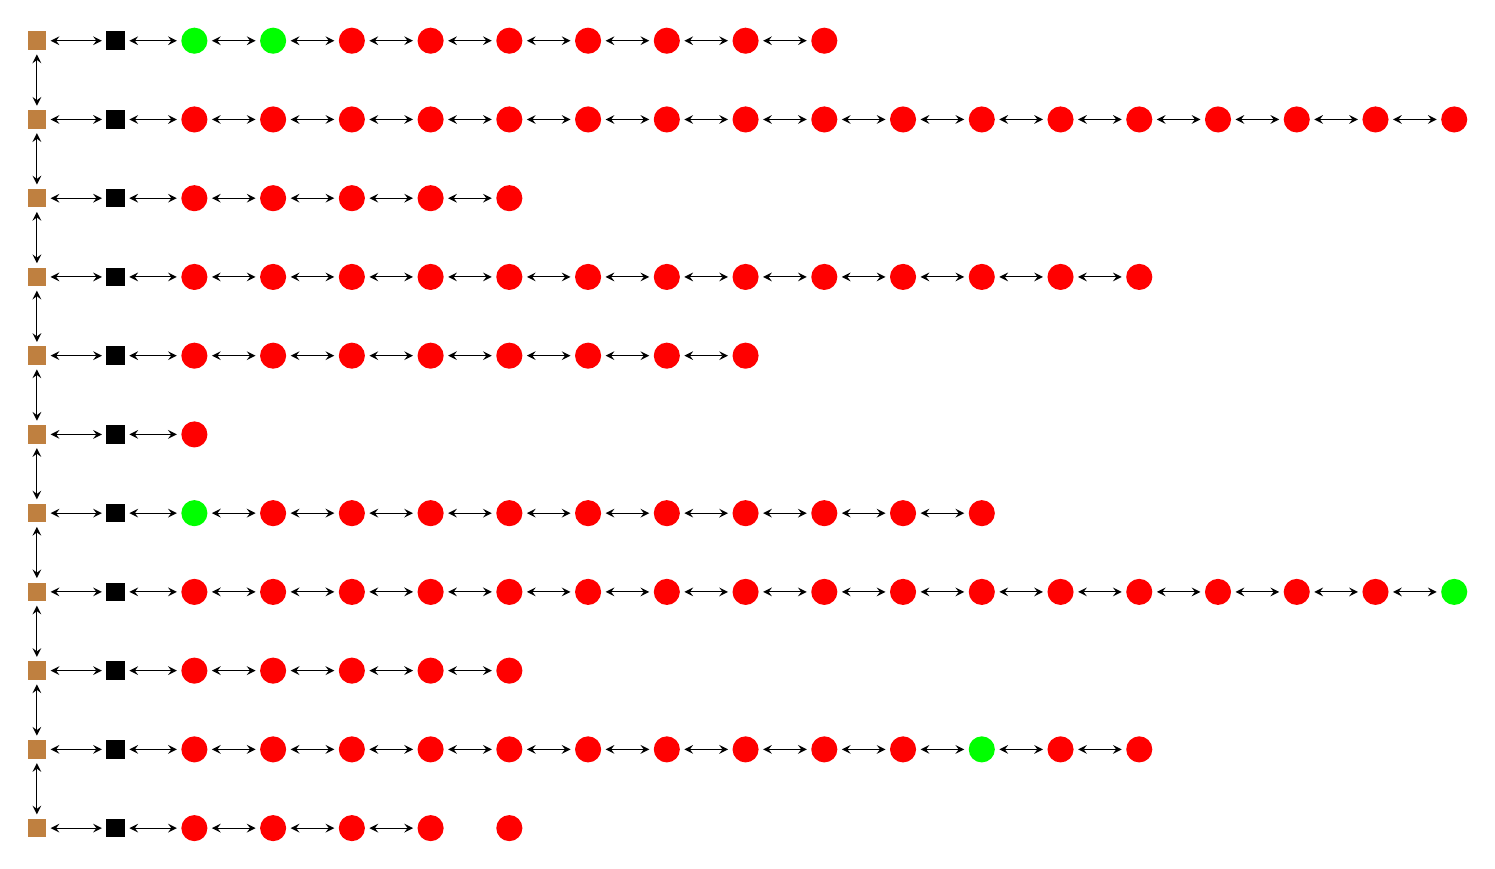
\begin{tikzpicture}[rotate=270,font=\tiny,
   oc/.style={fill=black,rectangle,minimum size=0.01cm,font=\tiny},
     feeder/.style={fill=brown,rectangle,minimum size=0.005cm,font=\tiny},
   Producer/.style={fill=green,circle,minimum size=0.01cm},
     Consumer/.style={fill=red,circle,minimum size=0.01cm},
   Connection/.style={<->, >=stealth, shorten <=0.05cm, shorten >=0.05cm}]
 \draw node[oc] (oc1) at (-5,0){};
 \draw node[oc] (oc2) at (-4,0){};
 \draw node[oc] (oc3) at (-3,0){};
 \draw node[oc] (oc4)  at (-2,0){};
 \draw node[oc](oc5)  at (-1,0){};
 \draw node[oc] (oc6)  at (0,0){};
 \draw node[oc] (oc7) at (1,0){};
 \draw node[oc] (oc8)  at (2,0){};
 \draw node[oc] (oc9) at (3,0){};
 \draw node[oc] (oc10) at (4,0){};
 \draw node[oc] (oc11) at (5,0){};

 \draw node[feeder] (feeder1) at (-5,-1){};
 \draw node[feeder] (feeder2) at (-4,-1){};
 \draw node[feeder] (feeder3) at (-3,-1){};
 \draw node[feeder] (feeder4)  at (-2,-1){};
 \draw node[feeder](feeder5)  at (-1,-1){};
 \draw node[feeder] (feeder6)  at (0,-1){};
 \draw node[feeder] (feeder7) at (1,-1){};
 \draw node[feeder] (feeder8)  at (2,-1){};
 \draw node[feeder] (feeder9) at (3,-1){};
 \draw node[feeder] (feeder10) at (4,-1){};
 \draw node[feeder] (feeder11) at (5,-1){};

 \draw [Connection] (feeder1) to (feeder2);
 \draw [Connection] (feeder2) to (feeder3);
 \draw [Connection] (feeder3) to (feeder4);
 \draw [Connection] (feeder4) to (feeder5);
 \draw [Connection] (feeder5) to (feeder6);
 \draw [Connection] (feeder6) to (feeder7);
 \draw [Connection] (feeder7) to (feeder8);
 \draw [Connection] (feeder8) to (feeder9);
 \draw [Connection] (feeder9) to (feeder10);
 \draw [Connection] (feeder10) to (feeder11);

\draw [Connection] (feeder1) to (oc1);
\draw [Connection] (feeder2) to (oc2);
\draw [Connection] (feeder3) to (oc3);
\draw [Connection] (feeder4) to (oc4);
\draw [Connection] (feeder5) to (oc5);
\draw [Connection] (feeder6) to (oc6);
\draw [Connection] (feeder7) to (oc7);
\draw [Connection] (feeder8) to (oc8);
\draw [Connection] (feeder9) to (oc9);
\draw [Connection] (feeder10) to (oc10);
\draw [Connection] (feeder11) to (oc11);


 \foreach \pos in {1,2} {
   \node [Producer] (p10\pos)at (-5,\pos) {};
 }

 \foreach \pos in {3,4,5,6,7,8,9} {
   \node [Consumer] (c10\pos)at (-5,\pos) {};
 }

 \foreach \pos in {1,2,3,4,5,6,7,8,9,10,11,12,13,14,15,16,17} {
   \node [Consumer] (c20\pos)at (-4,\pos) {};
 }

 \foreach \pos in {1,2,3,4,5} {
   \node [Consumer] (c30\pos)at (-3,\pos) {};
 }


 \foreach \pos in {1,2,3,4,5,6,7,8,9,10,11,12,13} {
   \node [Consumer] (c40\pos)at (-2,\pos) {};
 }


 \foreach \pos in {1,2,3,4,5,6,7,8} {
   \node [Consumer] (c50\pos)at (-1,\pos) {};
 }


 \foreach \pos in {1} {
   \node [Consumer] (c60\pos)at (0,\pos) {};
 }


 \foreach \pos in {1} {
   \node [Producer] (p70\pos)at (1,\pos) {};
 }


 \foreach \pos in {2,3,4,5,6,7,8,9,10,11} {
   \node [Consumer] (c70\pos)at (1,\pos) {};
 }


 \foreach \pos in {17} {
   \node [Producer] (p80\pos)at (2,\pos) {};
 }

 \foreach \pos in {1,2,3,4,5,6,7,8,9,10,11,12,13,14,15,16} {
   \node [Consumer] (c80\pos)at (2,\pos) {};
 }

 \foreach \pos in {1,2,3,4,5} {
   \node [Consumer] (c90\pos)at (3,\pos) {};
 }

 \foreach \pos in {11} {
   \node [Producer] (p100\pos)at (4,\pos) {};
 }

 \foreach \pos in {1,2,3,4,5,6,7,8,9,10,12,13} {
   \node [Consumer] (c100\pos)at (4,\pos) {};
 }

 \foreach \pos in {1,2,3,4,5} {
   \node [Consumer] (c110\pos)at (5,\pos) {};
 }


 \draw [Connection] (oc1) to (p101);
 \draw [Connection] (p101) to (p102);
 \draw [Connection] (p102) to (c103);
 \draw [Connection] (c103) to (c104);
 \draw [Connection] (c104) to (c105);
 \draw [Connection] (c105) to (c106);
 \draw [Connection] (c106) to (c107);
 \draw [Connection] (c107) to (c108);
 \draw [Connection] (c108) to (c109);
 
\draw [Connection] (oc2) to (c201);
\draw [Connection] (c201) to (c202);
\draw [Connection] (c202) to (c203);
\draw [Connection] (c203) to (c204);
\draw [Connection] (c204) to (c205);
\draw [Connection] (c205) to (c206);
\draw [Connection] (c206) to (c207);
\draw [Connection] (c207) to (c208);
\draw [Connection] (c208) to (c209);
\draw [Connection] (c209) to (c2010);
\draw [Connection] (c2010) to (c2011);
\draw [Connection] (c2011) to (c2012);
\draw [Connection] (c2012) to (c2013);
\draw [Connection] (c2013) to (c2014);
\draw [Connection] (c2014) to (c2015);
\draw [Connection] (c2015) to (c2016);
\draw [Connection] (c2016) to (c2017);

\draw [Connection] (oc3) to (c301);
\draw [Connection] (c301) to (c302);
\draw [Connection] (c302) to (c303);
\draw [Connection] (c303) to (c304);
\draw [Connection] (c304) to (c305);

\draw [Connection] (oc4) to (c401);
\draw [Connection] (c401) to (c402);
\draw [Connection] (c402) to (c403);
\draw [Connection] (c403) to (c404);
\draw [Connection] (c404) to (c405);
\draw [Connection] (c405) to (c406);
\draw [Connection] (c406) to (c407);
\draw [Connection] (c407) to (c408);
\draw [Connection] (c408) to (c409);
\draw [Connection] (c409) to (c4010);
\draw [Connection] (c4010) to (c4011);
\draw [Connection] (c4011) to (c4012);
\draw [Connection] (c4012) to (c4013);

\draw [Connection] (oc5) to (c501);
\draw [Connection] (c501) to (c502);
\draw [Connection] (c502) to (c503);
\draw [Connection] (c503) to (c504);
\draw [Connection] (c504) to (c505);
\draw [Connection] (c505) to (c506);
\draw [Connection] (c506) to (c507);
\draw [Connection] (c507) to (c508);

\draw [Connection] (oc6) to (c601);

\draw [Connection] (oc7) to (p701);
\draw [Connection] (p701) to (c702);
\draw [Connection] (c702) to (c703);
\draw [Connection] (c703) to (c704);
\draw [Connection] (c704) to (c705);
\draw [Connection] (c705) to (c706);
\draw [Connection] (c706) to (c707);
\draw [Connection] (c707) to (c708);
\draw [Connection] (c708) to (c709);
\draw [Connection] (c709) to (c7010);
\draw [Connection] (c7010) to (c7011);

\draw [Connection] (oc8) to (c801);
\draw [Connection] (c801) to (c802);
\draw [Connection] (c802) to (c803);
\draw [Connection] (c803) to (c804);
\draw [Connection] (c804) to (c805);
\draw [Connection] (c805) to (c806);
\draw [Connection] (c806) to (c807);
\draw [Connection] (c807) to (c808);
\draw [Connection] (c808) to (c809);
\draw [Connection] (c809) to (c8010);
\draw [Connection] (c8010) to (c8011);
\draw [Connection] (c8011) to (c8012);
\draw [Connection] (c8012) to (c8013);
\draw [Connection] (c8013) to (c8014);
\draw [Connection] (c8014) to (c8015);
\draw [Connection] (c8015) to (c8016);
\draw [Connection] (c8016) to (p8017);

\draw [Connection] (oc9) to (c901);
\draw [Connection] (c901) to (c902);
\draw [Connection] (c902) to (c903);
\draw [Connection] (c903) to (c904);
\draw [Connection] (c904) to (c905);

\draw [Connection] (oc10) to (c1001);
\draw [Connection] (c1001) to (c1002);
\draw [Connection] (c1002) to (c1003);
\draw [Connection] (c1003) to (c1004);
\draw [Connection] (c1004) to (c1005);
\draw [Connection] (c1005) to (c1006);
\draw [Connection] (c1006) to (c1007);
\draw [Connection] (c1007) to (c1008);
\draw [Connection] (c1008) to (c1009);
\draw [Connection] (c1009) to (c10010);
\draw [Connection] (c10010) to (p10011);
\draw [Connection] (p10011) to (c10012);
\draw [Connection] (c10012) to (c10013);


\draw [Connection] (oc11) to (c1101);
\draw [Connection] (c1101) to (c1102);
\draw [Connection] (c1102) to (c1103);
\draw [Connection] (c1103) to (c1104);

 \end{tikzpicture}
 }
 \caption{Feeder diagram. Brown nodes are feeder junctions, numbered 1 to 11 from top to bottom.  Black nodes are the overcurrent relays, which ensure that the total power flowing in and out of the feeder is below 20 kW. The green nodes are the junction points for the producers ($5$), and the red nodes are junction points for the consumers ($97$). There are $102$ prosumers in total.}
 \label{fig:feeder}
 \end{figure}


\begin{figure}[t]
\centering
\begin{tikzpicture}
\begin{axis}[
  font=\footnotesize,
  width=\columnwidth,
  height=0.61\columnwidth,
  ymin=-1,
 legend columns=3, 
  legend style={font=\fontsize{5}{6}\selectfont,cells={align=left},text width=4.3em,text height=1.5ex,text depth=.5ex,row sep=0.1em},
  ymax=220,
grid=both,
    grid style={line width=.1pt, draw=gray!10},
    major grid style={line width=.2pt,draw=gray!50},
  xmin=-1,
  xmax=97,
  legend pos=north west,
  xlabel=Time,
  ylabel={[kWh]},
  ytick={0, 50, 100, 150, 200},
  xtick={0, 16, 32, 48, 64, 80, 95},
  xticklabels={0:00, 4:00, 8:00, 12:00, 16:00,  20:00, 23:45},
]
\addplot[no markers, solid, greenline, semithick] table[x expr=\coordindex, y=WithoutBattery,  comment chars={\%}, col sep=comma] {diagrams/interval-energy-traded.csv};
\addlegendentry{Total energy traded (Test A)};
\addplot[no markers, solid, blackLine, semithick] table[x expr=\coordindex, y=WithBattery5,  comment chars={\%}, col sep=comma] {diagrams/interval-energy-traded.csv};
\addlegendentry{Total energy traded (Test C)};
\addplot[no markers, solid, goldLine, semithick] table[x expr=\coordindex, y=WithBattery12,  comment chars={\%}, col sep=comma] {diagrams/interval-energy-traded.csv};
\addlegendentry{Total energy traded (Test D)};
\addplot[no markers, solid, blueLine, semithick] table[x expr=\coordindex, y=TotalProduction, comment chars={\%}] {diagrams/TotalProductionConsumption.csv};
\addlegendentry{Total production};
\addplot[no markers, solid, redLine, semithick] table[x expr=\coordindex, y=TotalConsumption, comment chars={\%}] {diagrams/TotalProductionConsumption.csv};
\addlegendentry{Total consumption};
\end{axis}
\end{tikzpicture}
\caption{Load profile (i.e., total consumption) and generation profile (i.e., total production) in kWh per 15 minute interval aggregated across the microgrid.  The graph also shows the energy traded per interval without battery (Test A),  and with battery Tests C and D (see Table \ref{table:test-parameters}). Note that the amount of energy traded can be lower than both demand and supply at the same time because of safety constraints, which limit the amount of energy that can flow out of the producers' feeders.}
\label{fig:profile}
% \vspace{-0.2in}
\end{figure}



\begin{figure}[ht]
\begin{tikzpicture}
\begin{axis}[
  font=\footnotesize,
  width=0.94\columnwidth,
  height=0.65\columnwidth,
  ymin=-0.2,
  ymax=10,
  xmin=28,
  xmax=95,
  ylabel={Energy [kWh]},
  xtick={0, 16, 32, 48, 64, 80, 95},
  xticklabels={0:00, 4:00, 8:00, 12:00, 16:00,  20:00, 23:45},
grid=both,
    grid style={line width=.1pt, draw=gray!10},
    major grid style={line width=.2pt,draw=gray!50},
]
\addplot[mark=*, mark size=0.5, solid, blueLine, semithick] table[x= startTime, y=Energy, comment chars={\%}] {diagrams/outputTestA.csv};
\end{axis}
\begin{axis}[
  font=\footnotesize,
  width=0.94\columnwidth,
  height=0.65\columnwidth,
  ymin=-1,
  ymax=50,
  xmin=28,
  xmax=95,
  xtick={},
  xticklabels={},
  ylabel={Offer length [intervals]},
  ytick={0, 10, 20, 30, 40, 50},
  axis y line*=right,
  legend pos=north east,
]
\addlegendimage{blueLine, semithick}
\addlegendentry{Energy}
\addplot[ybar interval,redLine] table[ x=startTime,y=Availability, comment chars={\%}] {diagrams/outputTestA.csv};
\addlegendentry{Offer length}
\end{axis}
\end{tikzpicture}
\caption{Energy offered in each time interval by the first prosumer of the first feeder when using a battery (blue line). The red bars indicate the number of contiguous intervals for which the offer is valid. The total battery capacity is 90 kWh. It is assumed that the battery charges at a rate of 10 kWh per interval. Producers are assumed to keep the battery available till the end of the test, which is the 95th interval. Consequently, the red bars taper off in consecutive intervals.}
\label{fig:batteryEffect}
\end{figure}

 
 \begin{figure}[ht]
	\centering		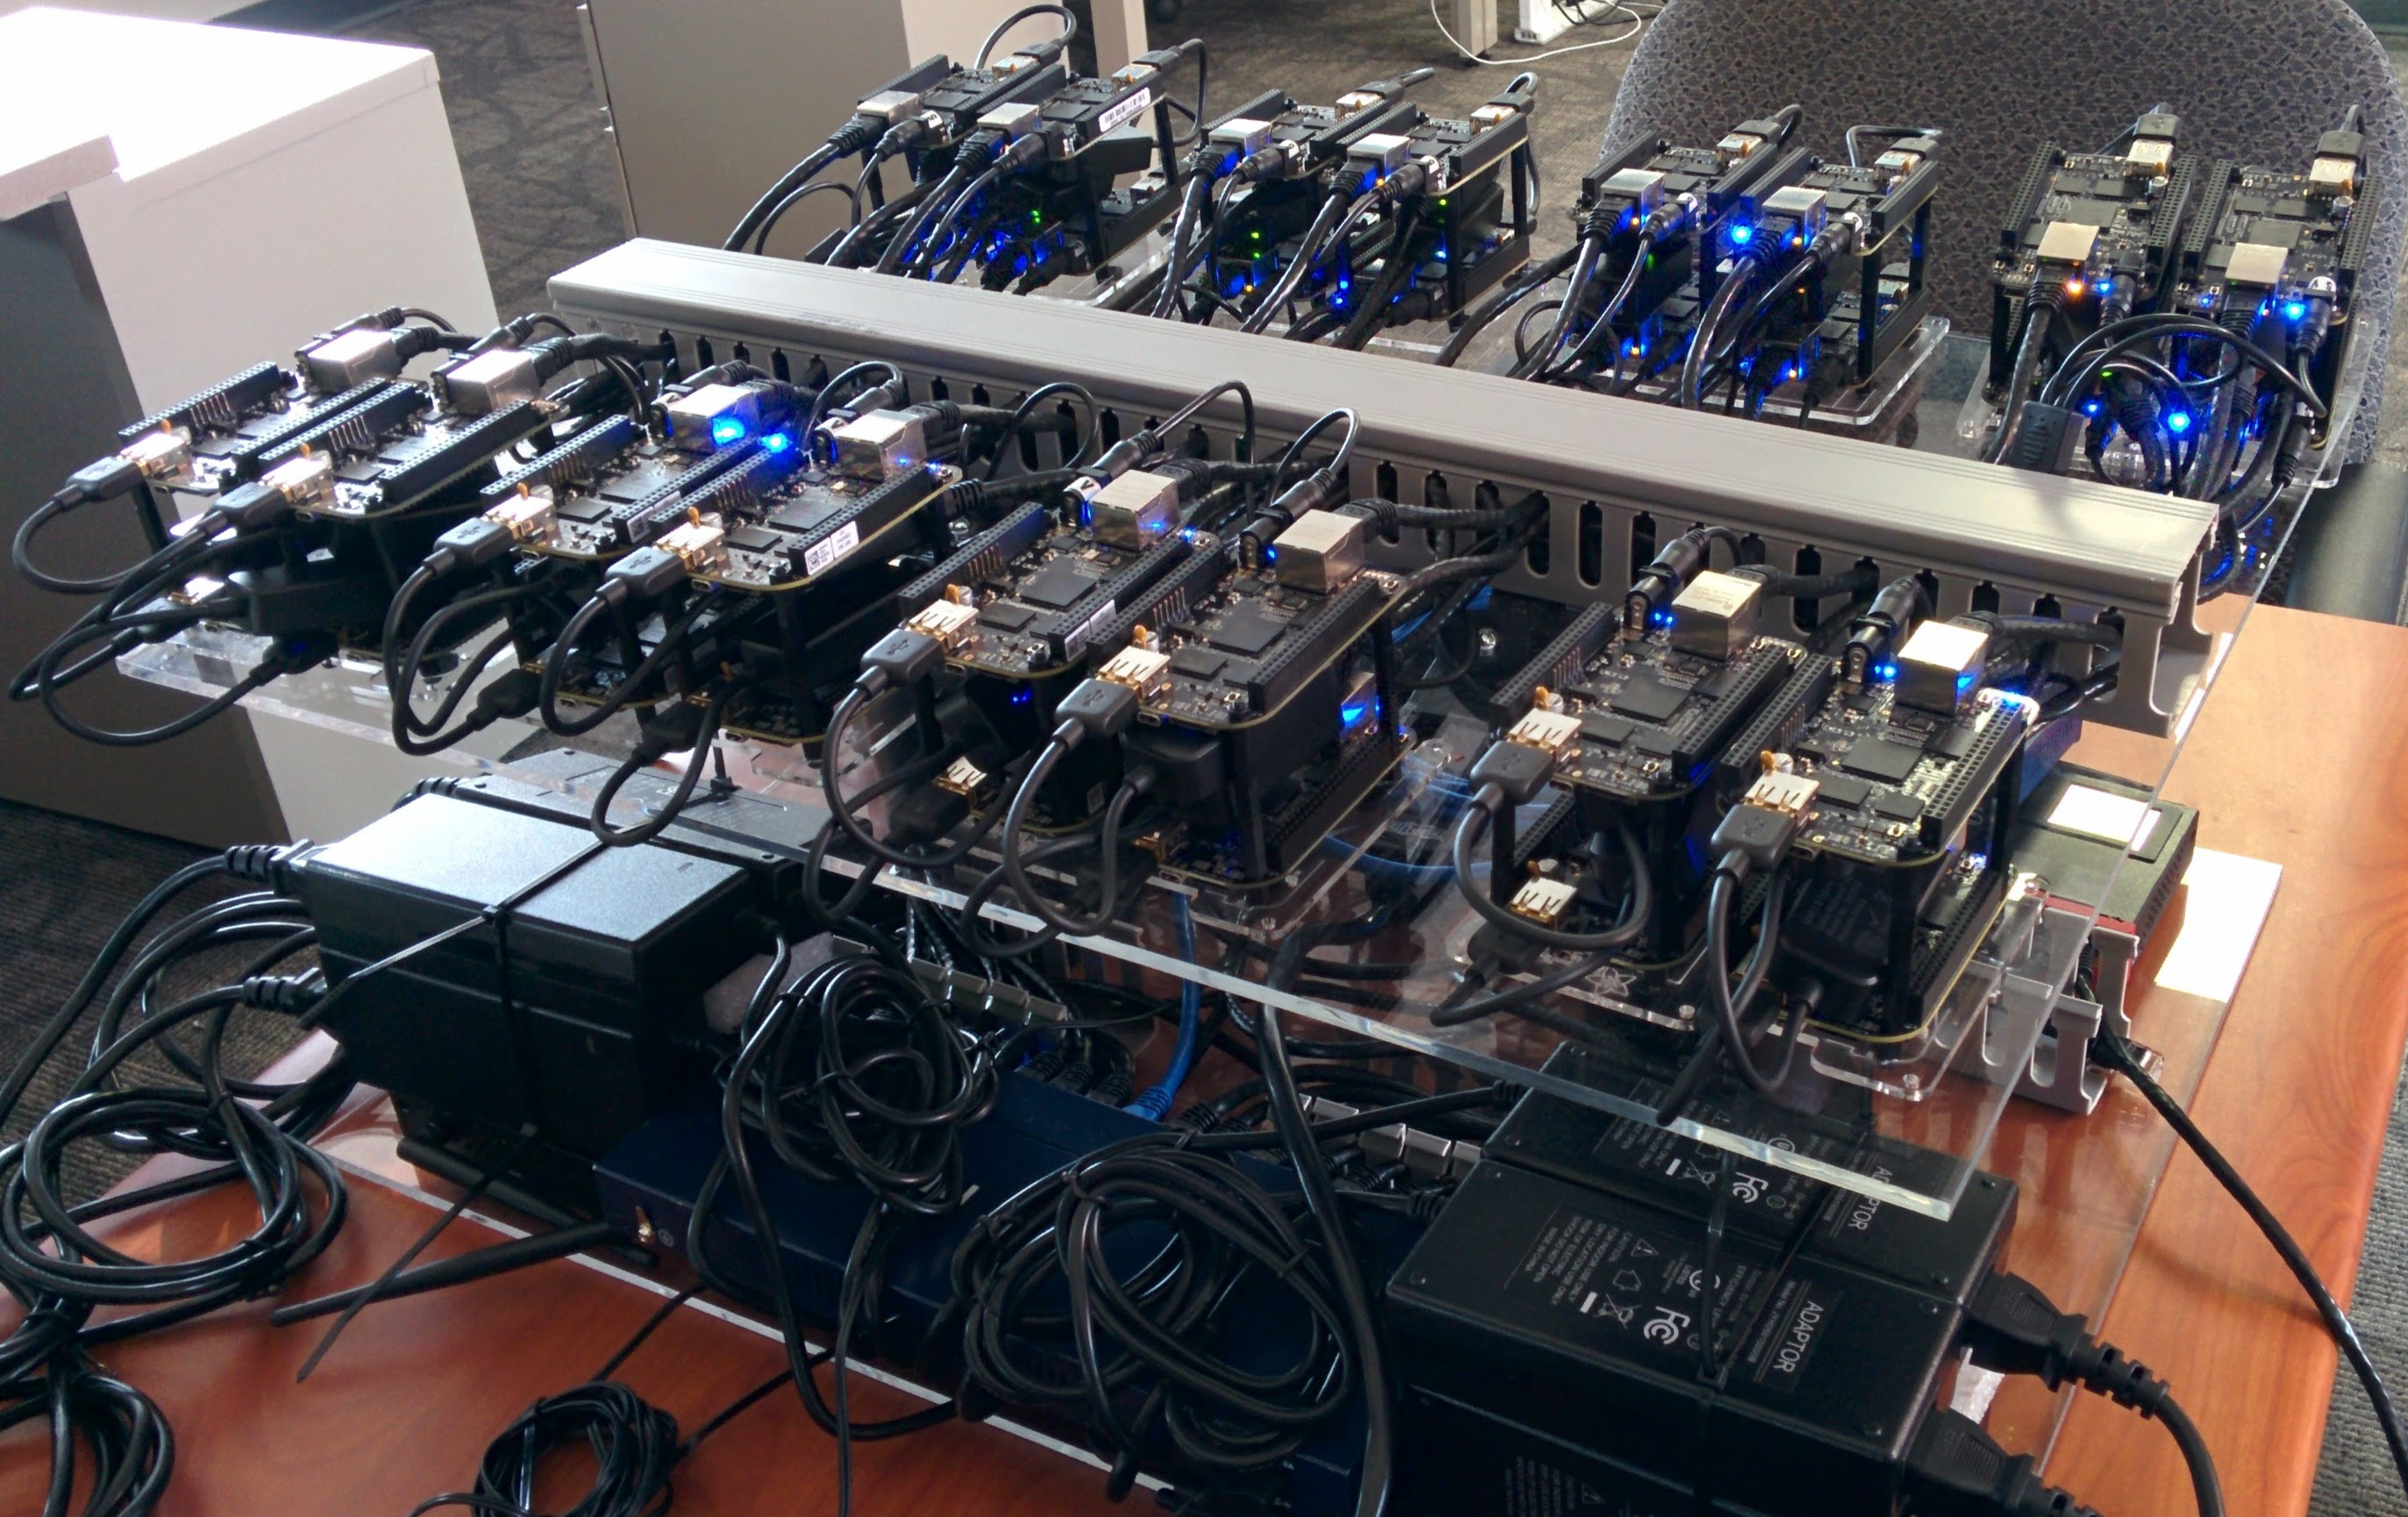
\includegraphics[width=1\columnwidth]{diagrams/testbed.jpg}
	\caption{Hardware test bed.}
   \label{fig:testbed_architecture}
\end{figure}


\begin{table}[ht]    
%\setlength{\tabcolsep}{4pt}
\caption{Parameter Values for Experiments (See Table \ref{tab:symbols})}
\label{table:test-parameters}  
\centering
\begin{tabular}{lllll}
& A  & B  & C  & D     \\ \cline{2-5} 
\multicolumn{1}{l|}{$\Delta$[m]}   & 15 & 15 & 15 & 15   \\
\multicolumn{1}{l|}{$\Delta_s$ [s]}   & 5 & 5 & 5 & 5   \\
\multicolumn{1}{l|}{$\hat{\Delta}$ [s]} & 120 & 120 & 120 & 120   \\
\multicolumn{1}{l|}{$L$}          & 2,3,5,7,10,13  & 2,3,7,10  & 5  & 13    \\
\multicolumn{1}{l|}{Battery}     & no & yes & yes & yes \\
\hline
\multicolumn{1}{l|}{Figure}     & \ref{fig:multihorizon} &\ref{fig:multihorizon} & \ref{fig:allocate1NRG},\ref{fig:time},\ref{fig:profile},\ref{fig:multihorizon} &  \ref{fig:profile},\ref{fig:multihorizon} 
\end{tabular}
\end{table}
